%%%% CAPÍTULO 2 - REVISÃO DA LITERATURA (OU REVISÃO BIBLIOGRÁFICA, ESTADO DA ARTE, ESTADO DO CONHECIMENTO)
%%
\chapter{Fundamentaç\~ao Te\'orica}\label{cap:fundamentacaoTeorica}

Este capítulo apresenta os conceitos relacionados a \gls{ca}. Primeiramente aborda-se a definição de \gls{ca}, seu uso em aplicações, os desafios enfrentados por essa estratégia e o detalhamento dos algoritmos de perforação de laço, memoização, aproximação de ponto flutuante e o descarte de tarefas. Apresenta também conceitos de Computação Paralela com um foco no uso da ferramenta OpenMP. Por fim, verificam-se trabalhos similares á presente pesquisa.

\section{Computação aproximada}\label{sec:compAprox}

A \gls{ca} consiste em um conjunto de técnicas aplicadas a cenários em que os resultados exatos não são estritamente necessários ou em que as aplicações apresentam resiliência suficiente para lidar com pequenas imprecisões em suas computações. Nessas situações, o uso de tais técnicas pode proporcionar ganhos significativos de desempenho e eficiência energética, mantendo a margem de erro em níveis reduzidos. Um exemplo é o uso de redes neurais para aproximar a divergência de \textit{branch} em instruções \gls{simd}, capaz de alcançar aceleração de até 14,8$\times$ com acurácia de 96\%~\cite{grigorian2015}. Por esse motivo, a \gls{ca} se mostra especialmente atraente em domínios como análise de dados, reconhecimento de padrões, processamento de imagens e sinais~\cite{mittal2016, chippa2013}.

As diferentes estratégias de aproximação podem ser classificadas conforme a camada em que são aplicadas na pilha computacional. No nível de \textit{hardware}, destacam-se técnicas que envolvem desde unidades funcionais aproximadas, como somadores, multiplicadores e divisores, até abordagens como \textit{overclocking}~\cite{leon2025a,leon2025b} e o uso de memórias aproximadas~\cite{fabricio2020}. No nível de \textit{software}, encontram-se estratégias mais generalistas, incluindo linguagens de programação aproximada~\cite{sampson2015}, \textit{runtimes} com suporte à aproximação~\cite{li2018,reis2024} e otimizações realizadas em nível de compilador~\cite{oliveira2024a,oliveira2024b}.

Apesar de seus benefícios, esse paradigma enfrenta desafios significativos. Em primeiro lugar, nem todas as aplicações são resilientes a erros em sua execução, o que limita o uso de técnicas mais generalistas e torna necessário definir métricas que permitam ajustar o grau de precisão desejado, seja pelo usuário ou pela própria aplicação~\cite{mittal2016}. Além disso, medir corretamente o nível de erro introduzido não é trivial, pois nem sempre está claro qual métrica deve ser aplicada à saída da aplicação~\cite{felzmann2021}. Outro ponto crítico é a propagação dos erros, que pode comprometer toda a execução: em alguns casos, a aplicação pode falhar abruptamente; em outros, concluir sua execução de forma aparentemente correta, mas com resultados significativamente distantes do esperado~\cite{fabricio2020}.

Diante disso é possível observar que a \gls{ca} não se restringe a um único método, mas a um conjunto de diversas estratégias que exploram diferentes aspectos da execução de um programa. Na subseção seguinte, são detalhados quatro dessas estratégias: perforação de laço, memoização, aproximação de ponto flutuante e o descarte de tarefas

\subsection{Perforação de laço}\label{subsec:perfLaco}

A perforação de laço é uma das técnicas mais simples de computação aproximada, cuja ideia central consiste em omitir determinadas iterações de um laço, reduzindo assim o tempo de execução de uma região de código~\cite{sidiroglou2011}.

Existem diferentes forma de implementar esse técnica, existem técnicas estáticas que são aplicadas em tempo de compilação e outras dinâmicas que permitem ajustar o grau de omissão em tempo de execução~\cite{li2018}.

Em ambos os casos é comum implementar essa otimização em laços que estão em um formato canônico~\cite{openmp2018}. A \autoref{code:loopCanon} apresenta a estrutura de um laço canônico, geralmente expresso na forma de um \texttt{for}, com três elementos principais:

\begin{itemize}
    \item \textbf{Expressão inicial:} define o limite inferior do laço, ou seja, o ponto em que a computação começa.
    \item \textbf{Expressão de teste:} geralmente um operador relacional que compara a variável de indução com o limite superior, delimitando o espaço de iterações.
    \item \textbf{Expressão de incremento/decremento:} atualiza a variável de indução e define o passo do laço.
\end{itemize}

\begin{sourcecode}[htb]\caption{\label{code:loopCanon}Estrutura de um laço canônico}
    \begin{lstlisting}[frame=single, language=C++]
        for (int i = 0; i < N; i += a) {
            ...
        }
    \end{lstlisting}
    \fonte{}
\end{sourcecode}

Uma técnica comumente encontrada na implementação desse algoritmo é a de incrementar a expressão de incremento, se considerarmos isso no \autoref{code:loopCanon} teríamos que a iterações deixariam de ser de \texttt{a} em \texttt{a} vezes, passaríamos a ter um incremento de \texttt{a + 1} vezes. Se considerarmos que inicialmente tem o valor \texttt{a = 1} ele passaria a ser \texttt{a = 2} e o comportamento do laço seguiria o que está na \autoref{fig:perfoMod}, nela temos que os blocos em branco seriam iterações não executadas enquanto os blocos em azul seriam iterações executadas.

Uma forma simples de aplicar a perforação de laço é alterar o passo do incremento da variável de indução, de modo que parte das iterações seja ignorada. No exemplo da \autoref{code:loopCanon}, se inicialmente o incremento for \texttt{a = 1} (\texttt{i++}), todas as iterações serão executadas. Entretanto, ao modificar o incremento para \texttt{a = 2} (\texttt{i += 2}), apenas metade delas será realizada, já que o laço passa a “pular” uma iteração a cada passo. Esse comportamento é ilustrado na \autoref{fig:perfoMod}, onde blocos em azul representam iterações executadas e blocos em branco representam iterações omitidas.

\begin{figure}[htb]
    \caption{Modelo de execução do algoritmo de perforação de laço}
    \label{fig:perfoMod}
    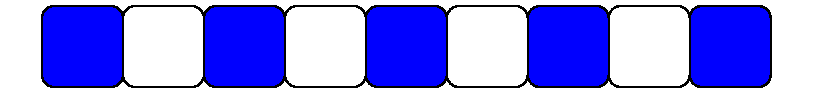
\includegraphics[scale=0.7]{Figuras/loop_perfo.pdf}
    \fonte{}
    \addcontentsline{loge}{figure}{\protect\numberline{\thefigure}Modelo de execução do algoritmo de perforação de laço.}
\end{figure}

\subsection{Memoização}\label{subsec:memo}

A memoização é tradicionalmente uma técnica associada à programação dinâmica que utiliza uma \textit{cache} de resultados para acelerar a execução de determinadas computações. Seu princípio consiste em armazenar os resultados de chamadas já realizadas, indexados pelas entradas correspondentes. Assim, quando a função é invocada novamente com os mesmos parâmetros, o valor previamente calculado é retornado diretamente, evitando a repetição da computação~\cite{michie1968}.

A memoização aproximada, também chamada de memoização temporal, estende esse conceito ao considerar tempo de execução e localização como critérios adicionais. Sua ideia principal é explorar o fato de que chamadas consecutivas a uma mesma função tendem a produzir resultados similares~\cite{tziantzioulis2018}.

Na prática, as saídas são armazenadas em uma estrutura de dados e reutilizadas seletivamente em chamadas subsequentes. As estratégias de \textit{cache} podem variar, incluindo modelos globais, específicos por função ou mesmo dependentes de contexto. O reuso é normalmente controlado por um limiar de tolerância, que avalia a variação das saídas: se os resultados permanecerem estáveis dentro desse limite, a função é considerada estável e, portanto, pode ser memoizada~\cite{tziantzioulis2018}.

\subsection{Aproximação de ponto flutuante}\label{subsec:pontoFlut}

A representação de números reais por meio de números de ponto flutuante envolvem aproximação por padrão devido a impossibilidade de representar valores contínuos, se torna impossível representar um número infinito com um número finito de \textit{bits}~\cite{monniaux2008}. Por esse motivo aritmética com números de ponto flutuante usualmente introduzem erros de aproximação que variam conforme a ordem de execução dessas operações, resultando em um valor completamente diferente do esperado. Um exemplo disso pode ser obervado na \autoref{fig:perfoMod}.

\begin{figure}[htb]
    \caption{Erro introduzido na aritmética de ponto flutuante.}
    \label{fig:floatPoint}
    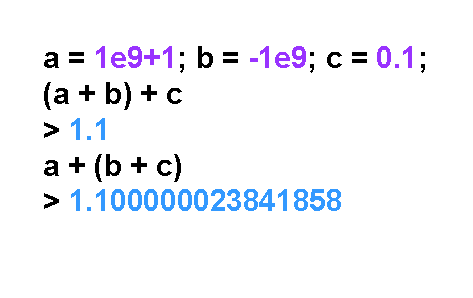
\includegraphics[scale=0.7]{Figuras/fastmath.pdf}
    \fonte{}
    \addcontentsline{loge}{figure}{\protect\numberline{\thefigure}Erro introduzido na aritmética de ponto flutuante.}
\end{figure}

Para reduzir este tipo de problema, compiladores usualmente evitam aplicar certas otimizações que podem amplificar o erro nesse tipo de operação. Porém, alguns compiladores como é o caso do \texttt{Clang} e o \texttt{GCC}, suportam a opção \texttt{--fast-math} que passa a permitir a aplicação dessas otimizações em todo um módulo de compilação~\cite{gccffast, clangffast}. E de maneira similar o \texttt{MSVC} suporta o uso da diretiva de compilação \texttt{\#pragma float\_control} para definir regiões do código que permitem o uso dessas otimizações em certas regiões decódigo~\cite{msvcfast}.

\subsection{Descarte de tarefas}\label{subsec:descTar}

O descarte de tarefas é um conceito abrangente que engloba diferentes técnicas de aproximação, incluindo, em alguns casos, a própria perforação de laço. Sua ideia central baseia-se em computações que podem ser divididas em unidades menores, chamadas tarefas, das quais uma parte delas é descartada~\cite{mittal2016}.

As implementações dessa técnica costumam adotar uma taxa de descarte, que define a fração de tarefas a serem eliminadas durante a execução do programa. A \autoref{fig:perfoMod} também pode ser utilizada para ilustrar esse mecanismo: os blocos brancos representam tarefas descartadas, enquanto os blocos azuis indicam as tarefas efetivamente executadas.

\section{Computação paralela}\label{sec:compParalela}


\section{Trabalhos relacionados}\label{sec:trabRelac}
\section{Considerações do capítulo}
